\section{Evaluation}
\label{sec:monitoring_wcet.evaluation}

% Toolflow
\begin{figure}
  \begin{center}
    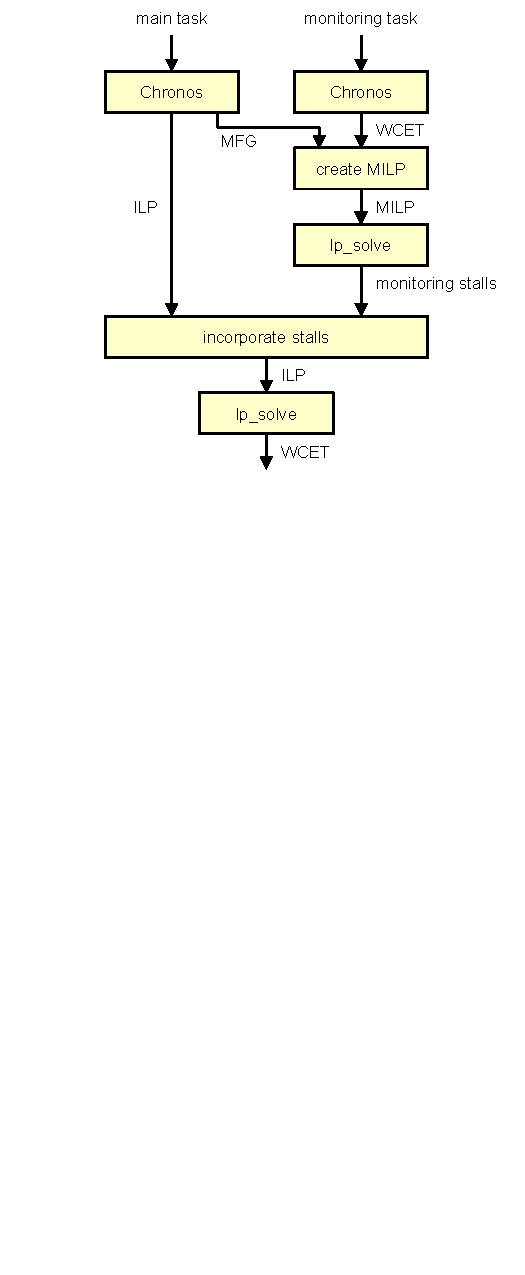
\includegraphics{monitoring_wcet/figs/toolflow.pdf}
    \caption{Toolflow for WCET estimation of parallel monitoring.}
    \label{fig:monitoring_wcet.evaluation.toolflow}
  \end{center}
\end{figure}

\subsection{Experimental Setup}

Our toolflow for the proposed WCET method is shown in
Figure~\ref{fig:monitoring_wcet.evaluation.toolflow}. We first use Chronos
\cite{chronos-tool}, an open source WCET tool, to estimate the WCET for the
main task and the monitoring tasks. We also modified Chronos to produce a MFG
of the main task. This MFG and the monitoring task WCET are used to produce an
MILP formulation as in Section \ref{sec:monitoring_wcet.wcet}. This MILP
problem is solved using lp\_solve \cite{lpsolve}, which produces the worst-case
monitoring stall cycles for each forwarded instruction. These monitoring stalls
are combined into the ILP formulation that is originally generated for the main
task to estimate the overall WCET with parallel run-time monitoring. Although
we use Chronos and lp\_solve for our implementation, these components can be
replaced with any WCET estimation tool and LP solver respectively.

To evaluate the effectiveness of our WCET scheme, we compared its estimate with
a simple WCET bound from sequential monitoring
(Section~\ref{sec:monitoring_wcet.wcet.sequential}) as well as simulation
results using the SimpleScalar architectural simulator \cite{simplescalar}.  In
addition to the WCET estimates with monitoring, we also compared the results
with the WCET of the main task without monitoring, using both Chronos and
simulations. 

For the experiments, we configured Chronos and SimpleScalar to model simple
processing cores that execute one instruction per cycle for both main and
monitoring cores and used an 8-entry FIFO.  This configuration represents
typical embedded microcontrollers, and is designed to focus on the impact of
parallel run-time monitoring by removing complex features such as branch
prediction and caches.  In the evaluation, we used seven benchmarks from the
M\"alardalen WCET benchmark suite \cite{malardalen} and two monitoring
techniques: uninitialized memory checks (UMC) and control flow protection
(CFP).  UMC detects a software bug that reads memory without a write.  CFP
protects a program's control flow by checking a target address on each control
transfer \cite{arora-runtime05}. In this technique, a compiler determines a set
of valid targets for each branch and jump in the main task.  This information
is stored on the monitoring core.  On a branch or jump, the monitoring core
ensures that the target is contained in the list of valid targets.
The WCET for UMC tasks was 7 cycles (i.e., $t_{M,max}$) and the WCET for CFP
was 9 cycles. Thus, the max monitoring loads were 56 and 72 cycles for UMC and
CFP respectively. These are relatively aggressive numbers that assume the
monitoring core is set up to automatically jump to the appropriate task based
on forwarded instruction type.

\subsection{WCET Results}

% Results
\begin{table*}
  \begin{center}
    \begin{scriptsize}
    % WCET results 

\begin{tabular}{|l|l||r|r|r|r|r|r|r|}
\hline

\multirow{2}{*}{\bf Monitoring}&\multirow{2}{*}{\bf Experiment}&\multicolumn{7}{c|}{\bf Benchmark}       \\ \cline{3-9}
&&\multicolumn{1}{c|}{\tt cnt}&\multicolumn{1}{c|}{\tt expint}&\multicolumn{1}{c|}{\tt fdct}&\multicolumn{1}{c|}{\tt fibcall}&\multicolumn{1}{c|}{\tt insertsort}&\multicolumn{1}{c|}{\tt matmult}&\multicolumn{1}{c|}{\tt ns} \\ \hline \hline
\multirow{2}{*}{None}&wcet-none&64531&3483&1805&245&598&133668&5951 \\ \cline{2-9}
&sim-none&62931&2293&1805&245&598&133668&5951 \\ \hline \hline
\multirow{3}{*}{UMC}&sequential-umc&103052&3591&4382&257&2489&357453&10338 \\ \cline{2-9}
&wcet-umc&64550&3498&3035&245&2083&256120&5953 \\ \cline{2-9}
&sim-umc&62931&2297&2564&245&1864&235120&5951 \\ \hline \hline
\multirow{3}{*}{CFP}&sequential-cfp&151732&11669&1976&794&1174&231507&18623 \\ \cline{2-9}
&wcet-cfp&93544&8984&1805&547&677&133668&13614 \\ \cline{2-9}
&sim-cfp&72540&5247&1805&382&598&133668&9824 \\ \hline

\end{tabular}

    \end{scriptsize}
    \caption{Estimated and observed WCET (clock cycles) with and without monitoring.}
    \label{tab:monitoring_wcet.evaluation.wcet}
  \end{center}
\end{table*}

Table~\ref{tab:monitoring_wcet.evaluation.wcet} shows the experimental results
for each benchmark under different configurations. The first set of rows show
the WCET estimate from Chronos ({\tt wcet-none}) and actual run-times from
simulations ({\tt sim-none}) without monitoring. The remaining rows show the
WCET for the UMC and CFP monitoring extensions. The results are shown for three
different approaches: a bound from sequential monitoring ({\tt sequential}),
our approach ({\tt wcet}), and simulations ({\tt sim}). The numbers indicate
the number of clock cycles.

% % Calculated ratios
% \begin{table*}
%   \begin{center}
%     \begin{tiny}
%     % WCET results 

\begin{tabular}{|lll||r|r|r|r|r|r|r||r|r|r|}
\hline

\multicolumn{3}{|c||}{\multirow{2}{*}{\bf Ratio}}  &\multicolumn{7}{c||}{\bf Benchmark}      &\multicolumn{1}{c|}{\multirow{2}{*}{\bf min}}&\multicolumn{1}{c|}{\multirow{2}{*}{\bf max}}&\multicolumn{1}{c|}{\multirow{2}{*}{\bf geomean}} \\ \cline{4-10}
&&&\multicolumn{1}{c|}{\tt cnt}&\multicolumn{1}{c|}{\tt expint}&\multicolumn{1}{c|}{\tt fdct}&\multicolumn{1}{c|}{\tt fibcall}&\multicolumn{1}{c|}{\tt insertsort}&\multicolumn{1}{c|}{\tt matmult}&\multicolumn{1}{c||}{\tt ns}&&& \\ \hline \hline
wcet-none&:&sim-none&1.03&1.52&1.00&1.00&1.00&1.00&1.00&1.00&1.52&1.07 \\ \hline
wcet-umc&:&sim-umc&1.03&1.52&1.18&1.00&1.12&1.09&1.00&1.00&1.52&1.12 \\ \hline
wcet-cfp&:&sim-cfp&1.29&1.71&1.00&1.43&1.13&1.00&1.39&1.00&1.71&1.26 \\ \hline \hline
sequential-umc&:&wcet-umc&1.60&1.03&1.44&1.05&1.19&1.40&1.74&1.03&1.74&1.33 \\ \hline
sequential-cfp&:&wcet-cfp&1.62&1.30&1.09&1.45&1.73&1.73&1.37&1.09&1.73&1.45 \\ \hline \hline
wcet-umc&:&wcet-none&1.00&1.00&1.68&1.00&3.48&1.92&1.00&1.00&3.48&1.41 \\ \hline
wcet-cfp&:&wcet-none&1.45&2.58&1.00&2.23&1.13&1.00&2.29&1.00&2.58&1.55 \\ \hline

\end{tabular}

%     \end{tiny}
%     \caption{Ratios comparing results from different experiments.} 
%     \label{tab:monitoring_wcet.evaluation.ratios}
%   \end{center}
% \end{table*}

% WCET vs. Simulation
\begin{figure}
  \begin{center}
    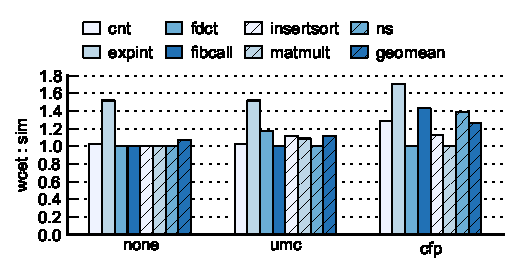
\includegraphics{monitoring_wcet/data/wcet-sim.pdf}
    \caption{Ratio of estimated WCET to observed WCET.}
    \label{fig:monitoring_wcet.evaluation.wcet-sim}
  \end{center}
\end{figure}
% Sequential WCET vs. Parallel WCET
\begin{figure}
  \begin{center}
    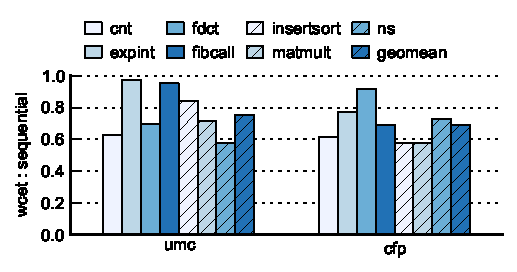
\includegraphics{monitoring_wcet/data/wcet-sequential.pdf}
    \caption{Ratio of WCET using our proposed method compared to assuming
    sequential monitoring.}
    \label{fig:monitoring_wcet.evaluation.wcet-sequential}
  \end{center}
\end{figure}
% Monitoring vs. None
\begin{figure}
  \begin{center}
    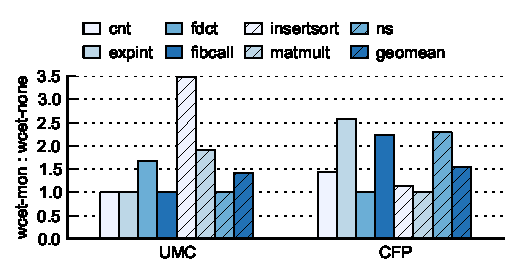
\includegraphics{monitoring_wcet/data/mon-none.pdf}
    \caption{Ratio of WCET with monitoring to WCET without monitoring.}
    \label{fig:monitoring_wcet.evaluation.mon-none}
  \end{center}
\end{figure}

Figure~\ref{fig:monitoring_wcet.evaluation.wcet-sim} shows the WCET estimates
from ILP/MILP formulations with the worst-case simulation cycles for each
monitoring setup.  The results show that the
analytical WCET estimates from our proposed scheme are larger than the observed
WCET by 0\% to 52\% for UMC and 0\% to 71\% for CFP, depending on the main
task. This difference is comparable to the case without parallel run-time
monitoring, where the analytical WCET from Chronos is larger than simulation
results by 0\% to 52\%.  In fact, for {\tt expint}, the majority of the
difference is from the WCET estimate of the main task rather than the effects
of monitoring.  This result suggests that our WCET approach is not
significantly more conservative than the baseline WCET tool for the main task.

Figure~\ref{fig:monitoring_wcet.evaluation.wcet-sequential} shows the WCET from
our proposed method normalized to the WCET calculated assuming sequential
monitoring.  For UMC, our approach shows up to a 43\%
reduction in WCET estimates over the simple bound. Similarly, for CFP, our
method shows up to a 42\% improvement.  These results demonstrate that modeling
the FIFO decoupling between the main and monitoring tasks is important for
obtaining tight WCET estimates of parallel monitoring. 

Finally, Figure~\ref{fig:monitoring_wcet.evaluation.mon-none}
compares the WCET estimates with and without run-time monitoring.  The results
show that the increase in WCET varies significantly depending on benchmark and
monitoring technique. Benchmarks with infrequent monitoring events (forwarded
instructions) show minimal overheads while ones with frequent monitoring can
see significant impacts.  Also, the benchmarks with large WCET increases differ
between UMC and CFP.  Therefore, when applying parallel run-time monitoring
techniques to real-time systems, a careful WCET analysis for the given tasks
and monitoring techniques needs to be performed. 

% The impact of run-time monitoring on the execution time in our experiments (up
% to 3.48x in UMC and 2.58x in CFP) is roughly in line with previous studies on
% multi-cores without any hardware support \cite{chen08-lba, nagarajan08-dift}.
% The performance overheads will be much lower for multi-cores with optimizations
% \cite{chen08-lba} or heterogeneous monitors \cite{flexcore-micro10}.  Our
% analysis technique does not depend on any specific monitoring core
% microarchitecture and is applicable to more optimized architectures.

%%%%%%%%%%%%%%%%%%%%%%%%%%%%%%%%%%%%%%%%%%%%%%%%%%
% lp_solve time
%%%%%%%%%%%%%%%%%%%%%%%%%%%%%%%%%%%%%%%%%%%%%%%%%%
\subsection{Time to Solve Linear Programming Problem}
\label{sec:monitoring_wcet.evaluation.lptime}

% lp_solve time
\begin{table*}
  \begin{center}
    \begin{footnotesize}
    % lp_solve run time

\begin{tabular}{|l||r|r|r|r|r|r|r|}
\hline

\multirow{2}{*}{\bf Solver Target}&\multicolumn{7}{c|}{\bf Benchmark}       \\ \cline{2-8}
&\multicolumn{1}{c|}{\tt cnt}&\multicolumn{1}{c|}{\tt expint}&\multicolumn{1}{c|}{\tt fdct}&\multicolumn{1}{c|}{\tt fibcall}&\multicolumn{1}{c|}{\tt insertsort}&\multicolumn{1}{c|}{\tt matmult}&\multicolumn{1}{c|}{\tt ns}\\ \hline \hline
stall-umc&17.789&6.256&21.733&0.043&0.390&161.796&3.655\\ \hline
stall-cfp&3.691&97.93&0.038&0.024&0.025&14.209&1.474\\ \hline \hline
sequential-umc&0.006&0.004&0.004&0.005&0.002&0.004&0.006\\ \hline
sequential-cfp&0.007&0.001&0.003&0.002&0.003&0.006&0.003\\ \hline \hline
wcet-none&0.003&0.003&0.004&0.002&0.002&0.002&0.001\\ \hline
wcet-umc&0.004&0.004&0.003&0.001&0.004&0.005&0.002\\ \hline
wcet-cfp&0.002&0.007&0.005&0.004&0.003&0.005&0.004\\ \hline

\end{tabular}

    \end{footnotesize}
    \caption{Running time of lp\_solve in seconds to determine worst-case stalls
    (stall), sequential bound (sequential), and worst-case execution times (wcet).}
    \label{tab:monitoring_wcet.evaluation.runtime}
  \end{center}
\end{table*}

In this section, we evaluate the running time of our analysis method.
The most time intensive portion of this analysis is solving of
the linear programming (LP) problem. For our experiments, we used lp\_solve
5.5.2.0 \cite{lpsolve} as our LP solver. These experiments were run on a 2.67
GHz Xeon E5430 quad-core processor with 4 GB of RAM. The running times for
lp\_solve are shown in Table~\ref{tab:monitoring_wcet.evaluation.runtime}.  The
first set of rows show the running time for determining the worst-case stalls
from the monitoring flow graph ({\tt stall}). The second set of rows show the
lp\_solve running time for finding the sequential bounds. The final set of rows
show the running time for determining the overall WCET ({\tt wcet}). For {\tt
wcet-umc} and {\tt wcet-cfp}, this is for the ILP problem given that the worst-case
stalls have already been found.

The running times for the {\tt sequential} cases and the {\tt wcet} cases are
very similar. This is because these cases are all solving essentially the same
problem with different numbers. That is, for a given benchmark, these different
cases are all solving a linear programming problem for the same control flow
graph (CFG). As a result, the number of variables and the set of constraints is
the same, though the WCET for each basic block changes depending on the
extension and the estimation method. 

The {\tt stall} cases, where we calculate the worst-case stalls using our
MILP-based method, have a longer running time. This is due to the fact that a
MFG has more nodes than its corresponding CFG. The increased number of nodes
also implies more variables and more constraints. An interesting direction for
future work would be to explore graph transformations to reduce the MFG size
and thus reduce the analysis time.

